\documentclass[pdftex]{article}
\usepackage[T1]{fontenc}
\usepackage[utf8]{inputenc}
\usepackage{graphicx}
\usepackage[font=scriptsize,labelfont=bf]{caption}
\usepackage{titling}

\setlength{\droptitle}{-15em}
\title{PHYS 721 Homework 5}
\author{Nick Tyler}
\date{}


\begin{document}
\captionsetup[figure]{aboveskip=-15pt}
\captionsetup[figure]{belowskip=15pt}
\maketitle
\begin{enumerate}
	\item Three Breit-Wigner curves are fitted to data for the decay $\phi \rightarrow K^{+} K^{-}$. 
		The first fit, in green, is the relativistic Breit-Wigner with a mass \\ dependent $\Gamma$, 
		$\Gamma = \Gamma_{0} \left( \frac{p}{p_0} \right)^3$. The second fit, in blue, is the relativistic Breit-Wigner 
		while the third, in red, is the Non-Relativistic Breit-Wigner curve. \

		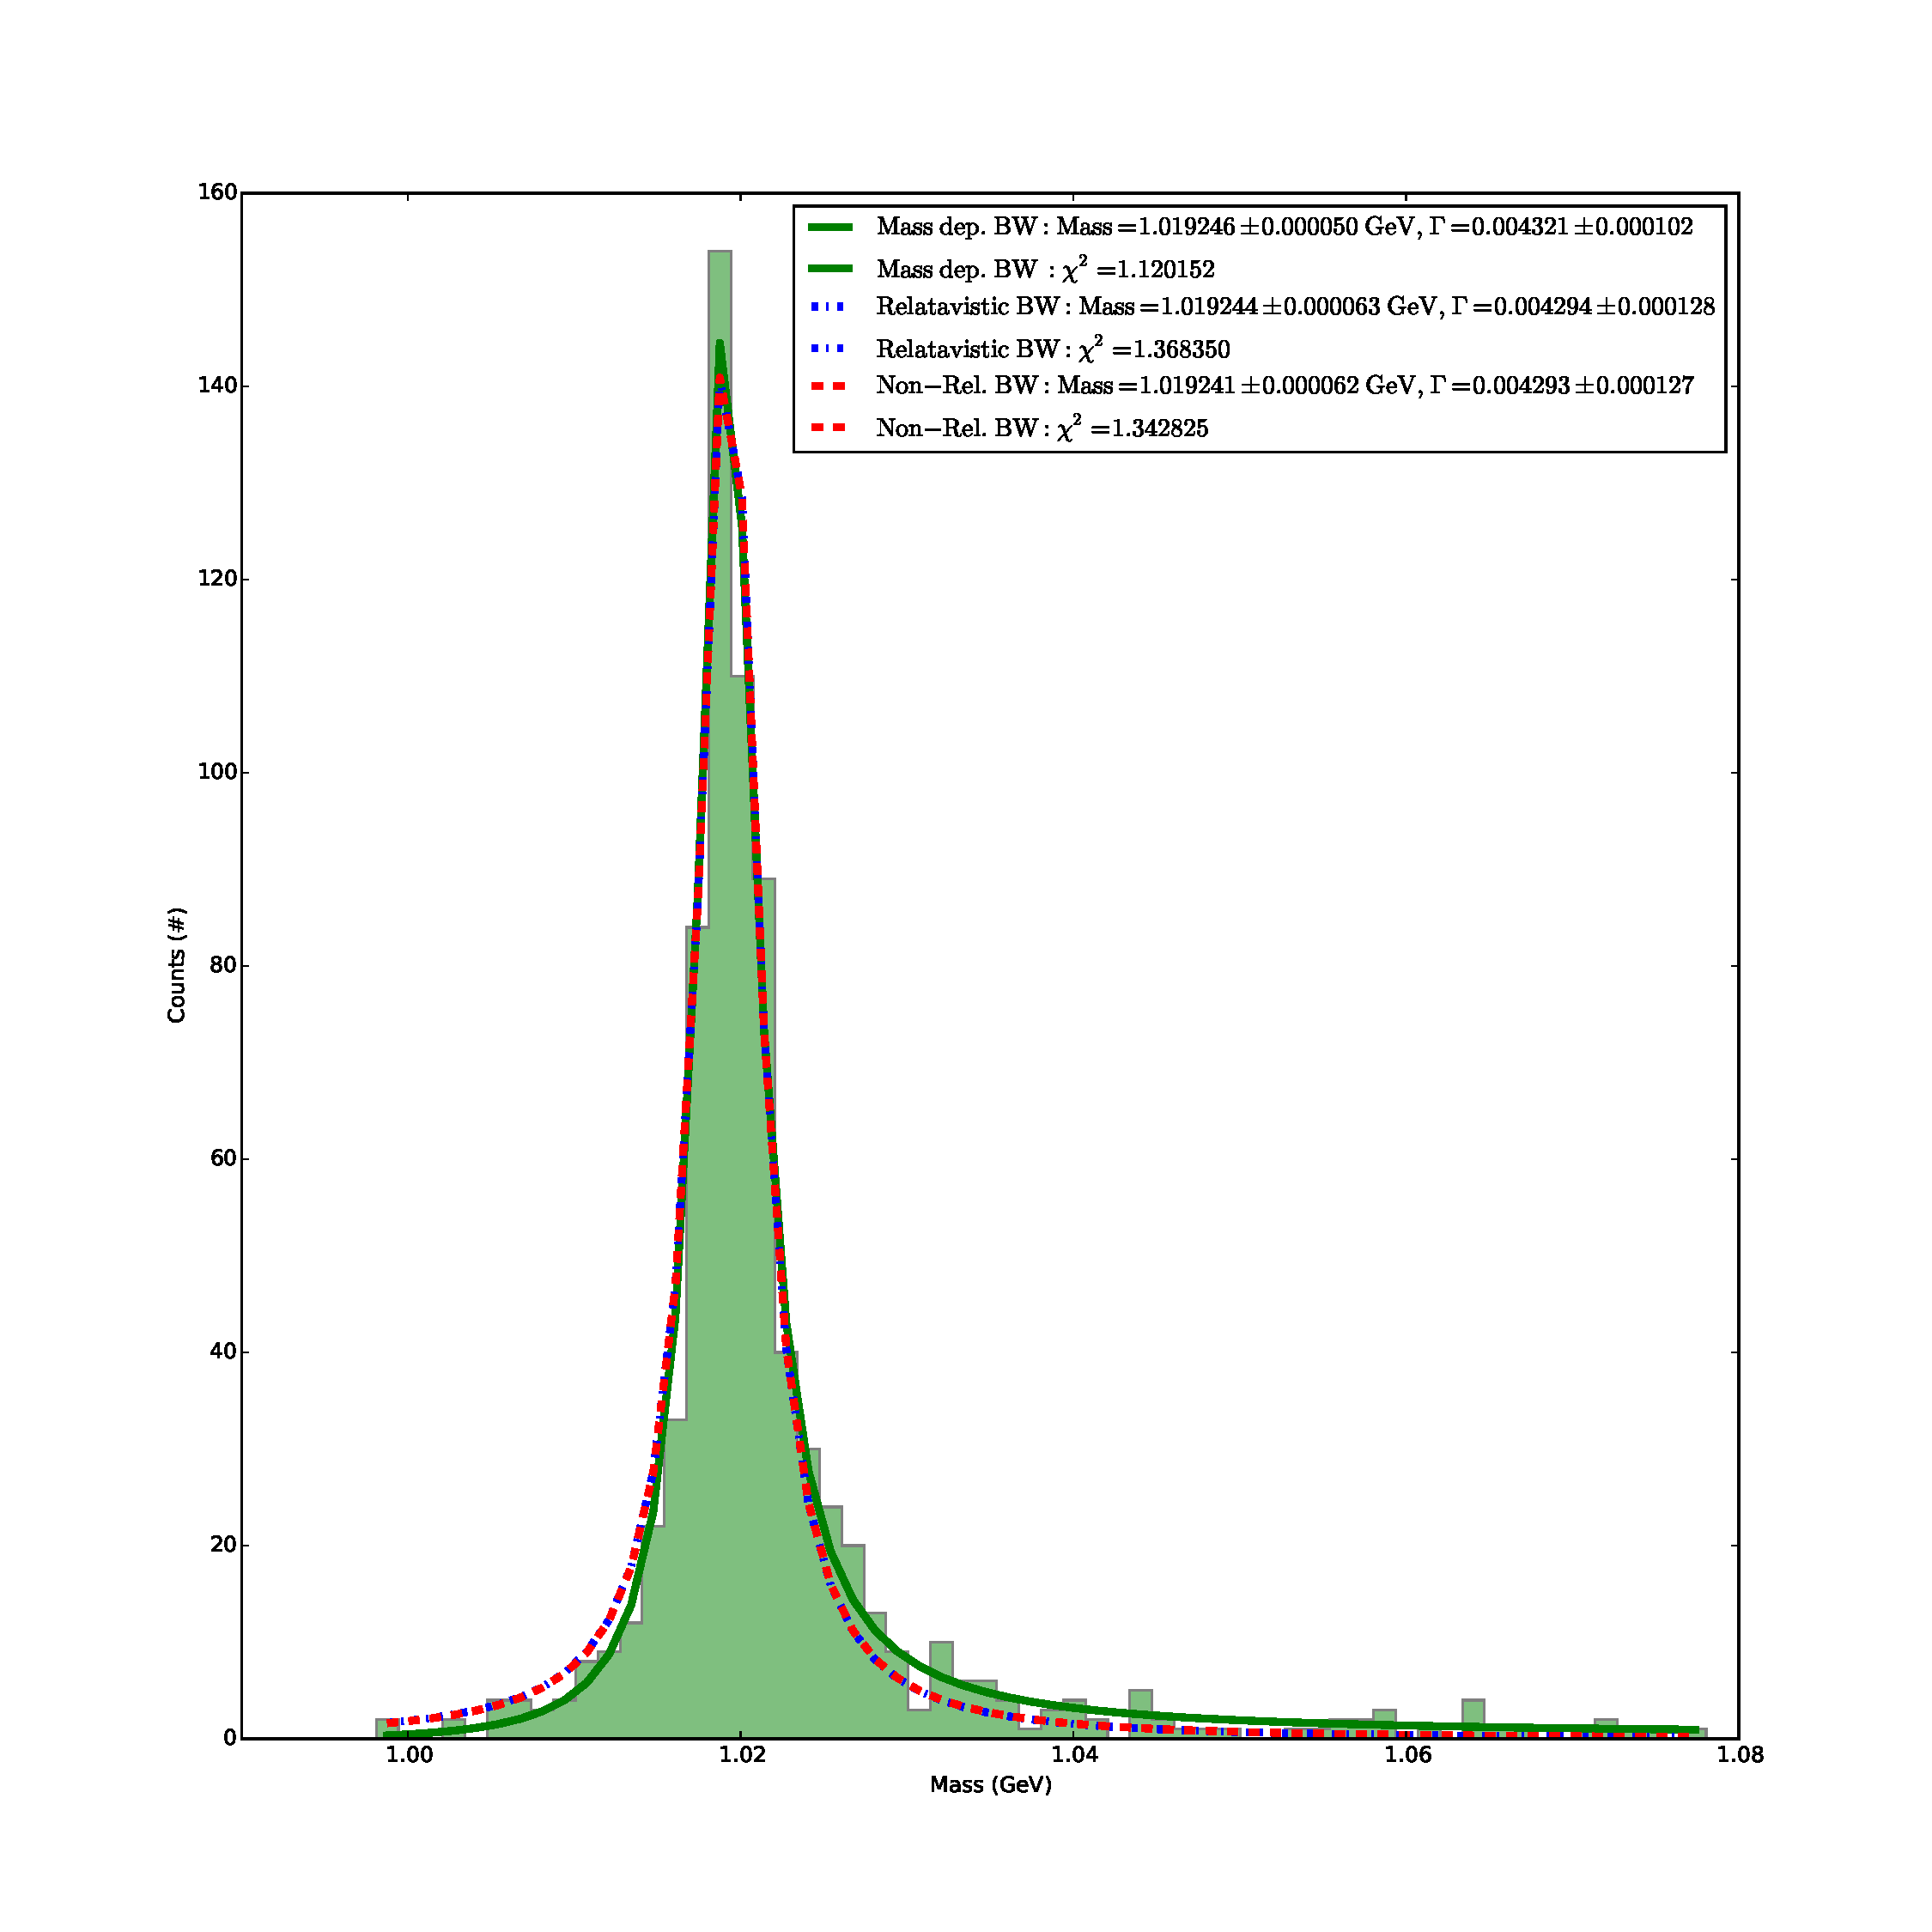
\includegraphics[scale=0.35]{Problem_1_and_2.pdf}\\
		\captionof{figure}{Three Breit-Wigner curves fit to data for, $\phi \rightarrow K^{+} K^{-}$}
		
	\pagebreak

	\item By looking at the $\chi^2$ values from figure one the first fit, the relativistic Breit-Wigner
		with mass dependent $\Gamma$ appears to give the best value. In order to determine which fit the data prefers one would need enough data to decrease the $\chi^2$ values close to one.  Enough values to give a $10\%$ difference in $\chi^2$ values would show that one fit was better than the other.


	\item The steps for problem one and two were also completed with a dataset with an equal amount of background data.
		The results are in the following figures.

		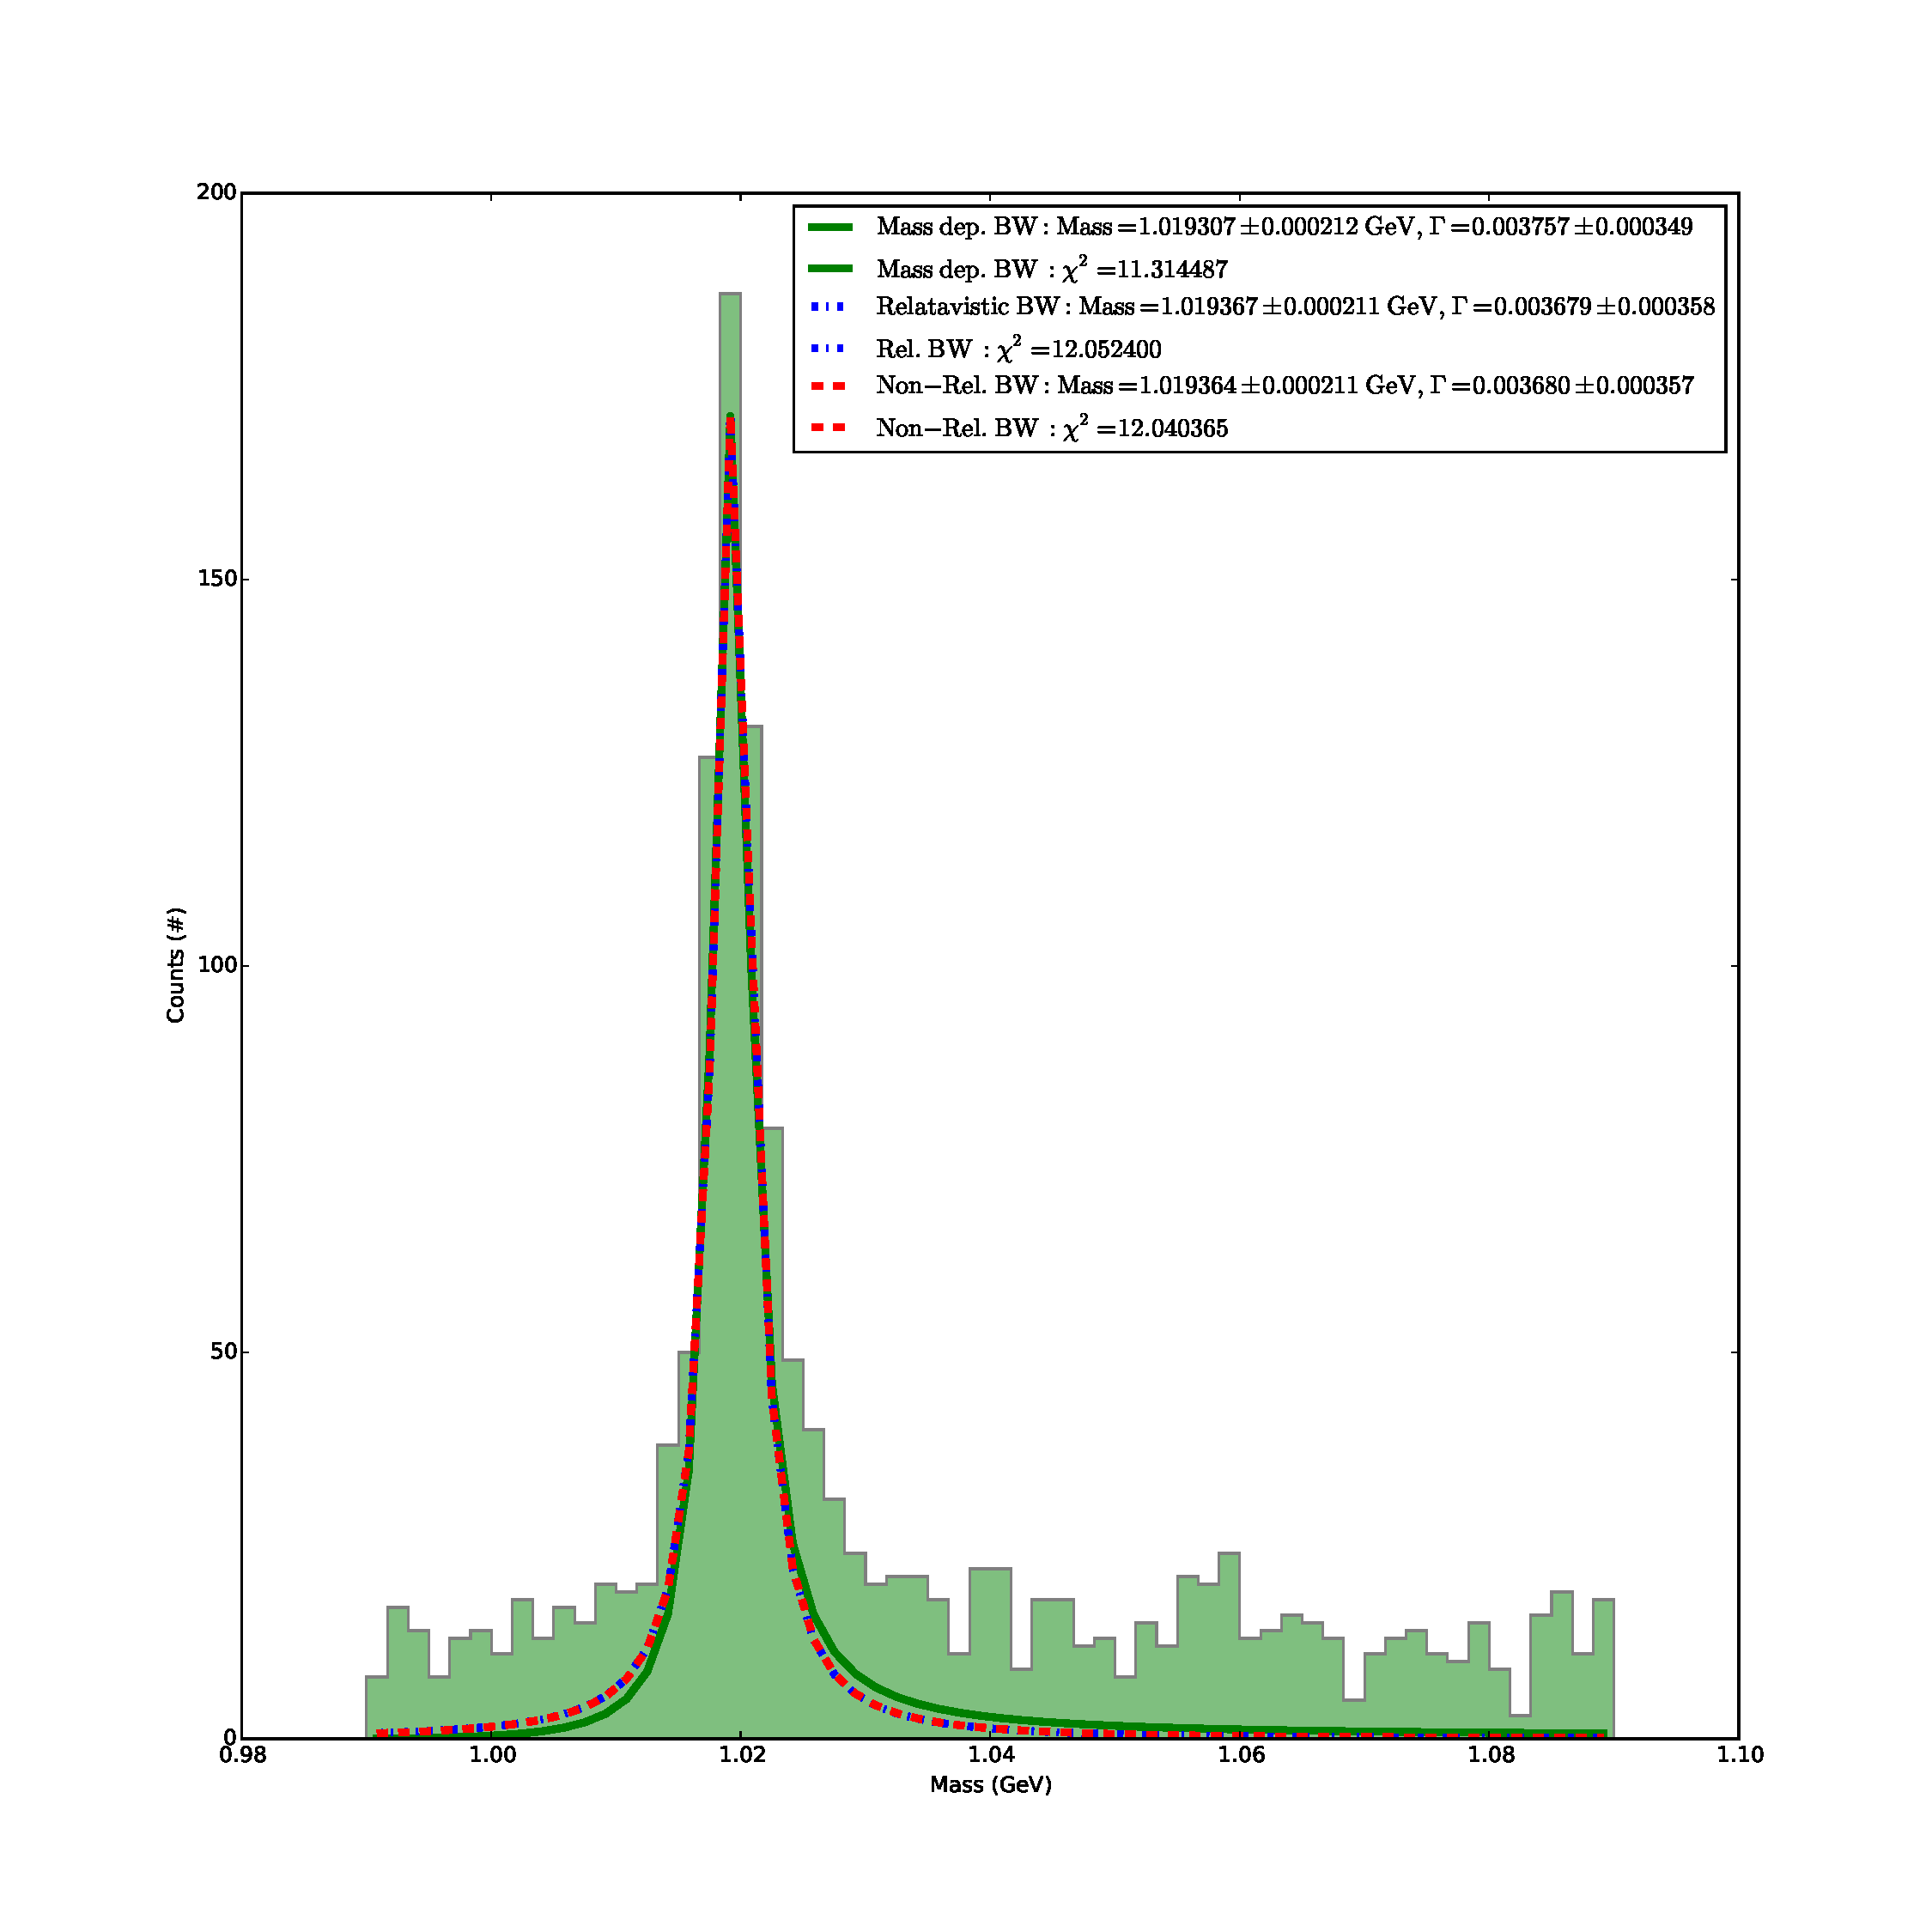
\includegraphics[scale=0.35]{Problem_3_nobackfit.pdf}
		\captionof{figure}{Three Breit-Wigner histograms with background for,
							$\phi \rightarrow K^{+} K^{-}$.
							The fit's used do not include a fit for the background events.}


		\ \ \ \ \ With the background added to the data the fits produce very poor results. The curves do not match the peak
		and the tails of the curves are much below the histogram. Also by looking at the $\chi^2$ values one can
		see that the fits are much poorer than the original fits without background. It is therefore important 
		to also model and fit the background along with the data as seen in figure 3.

		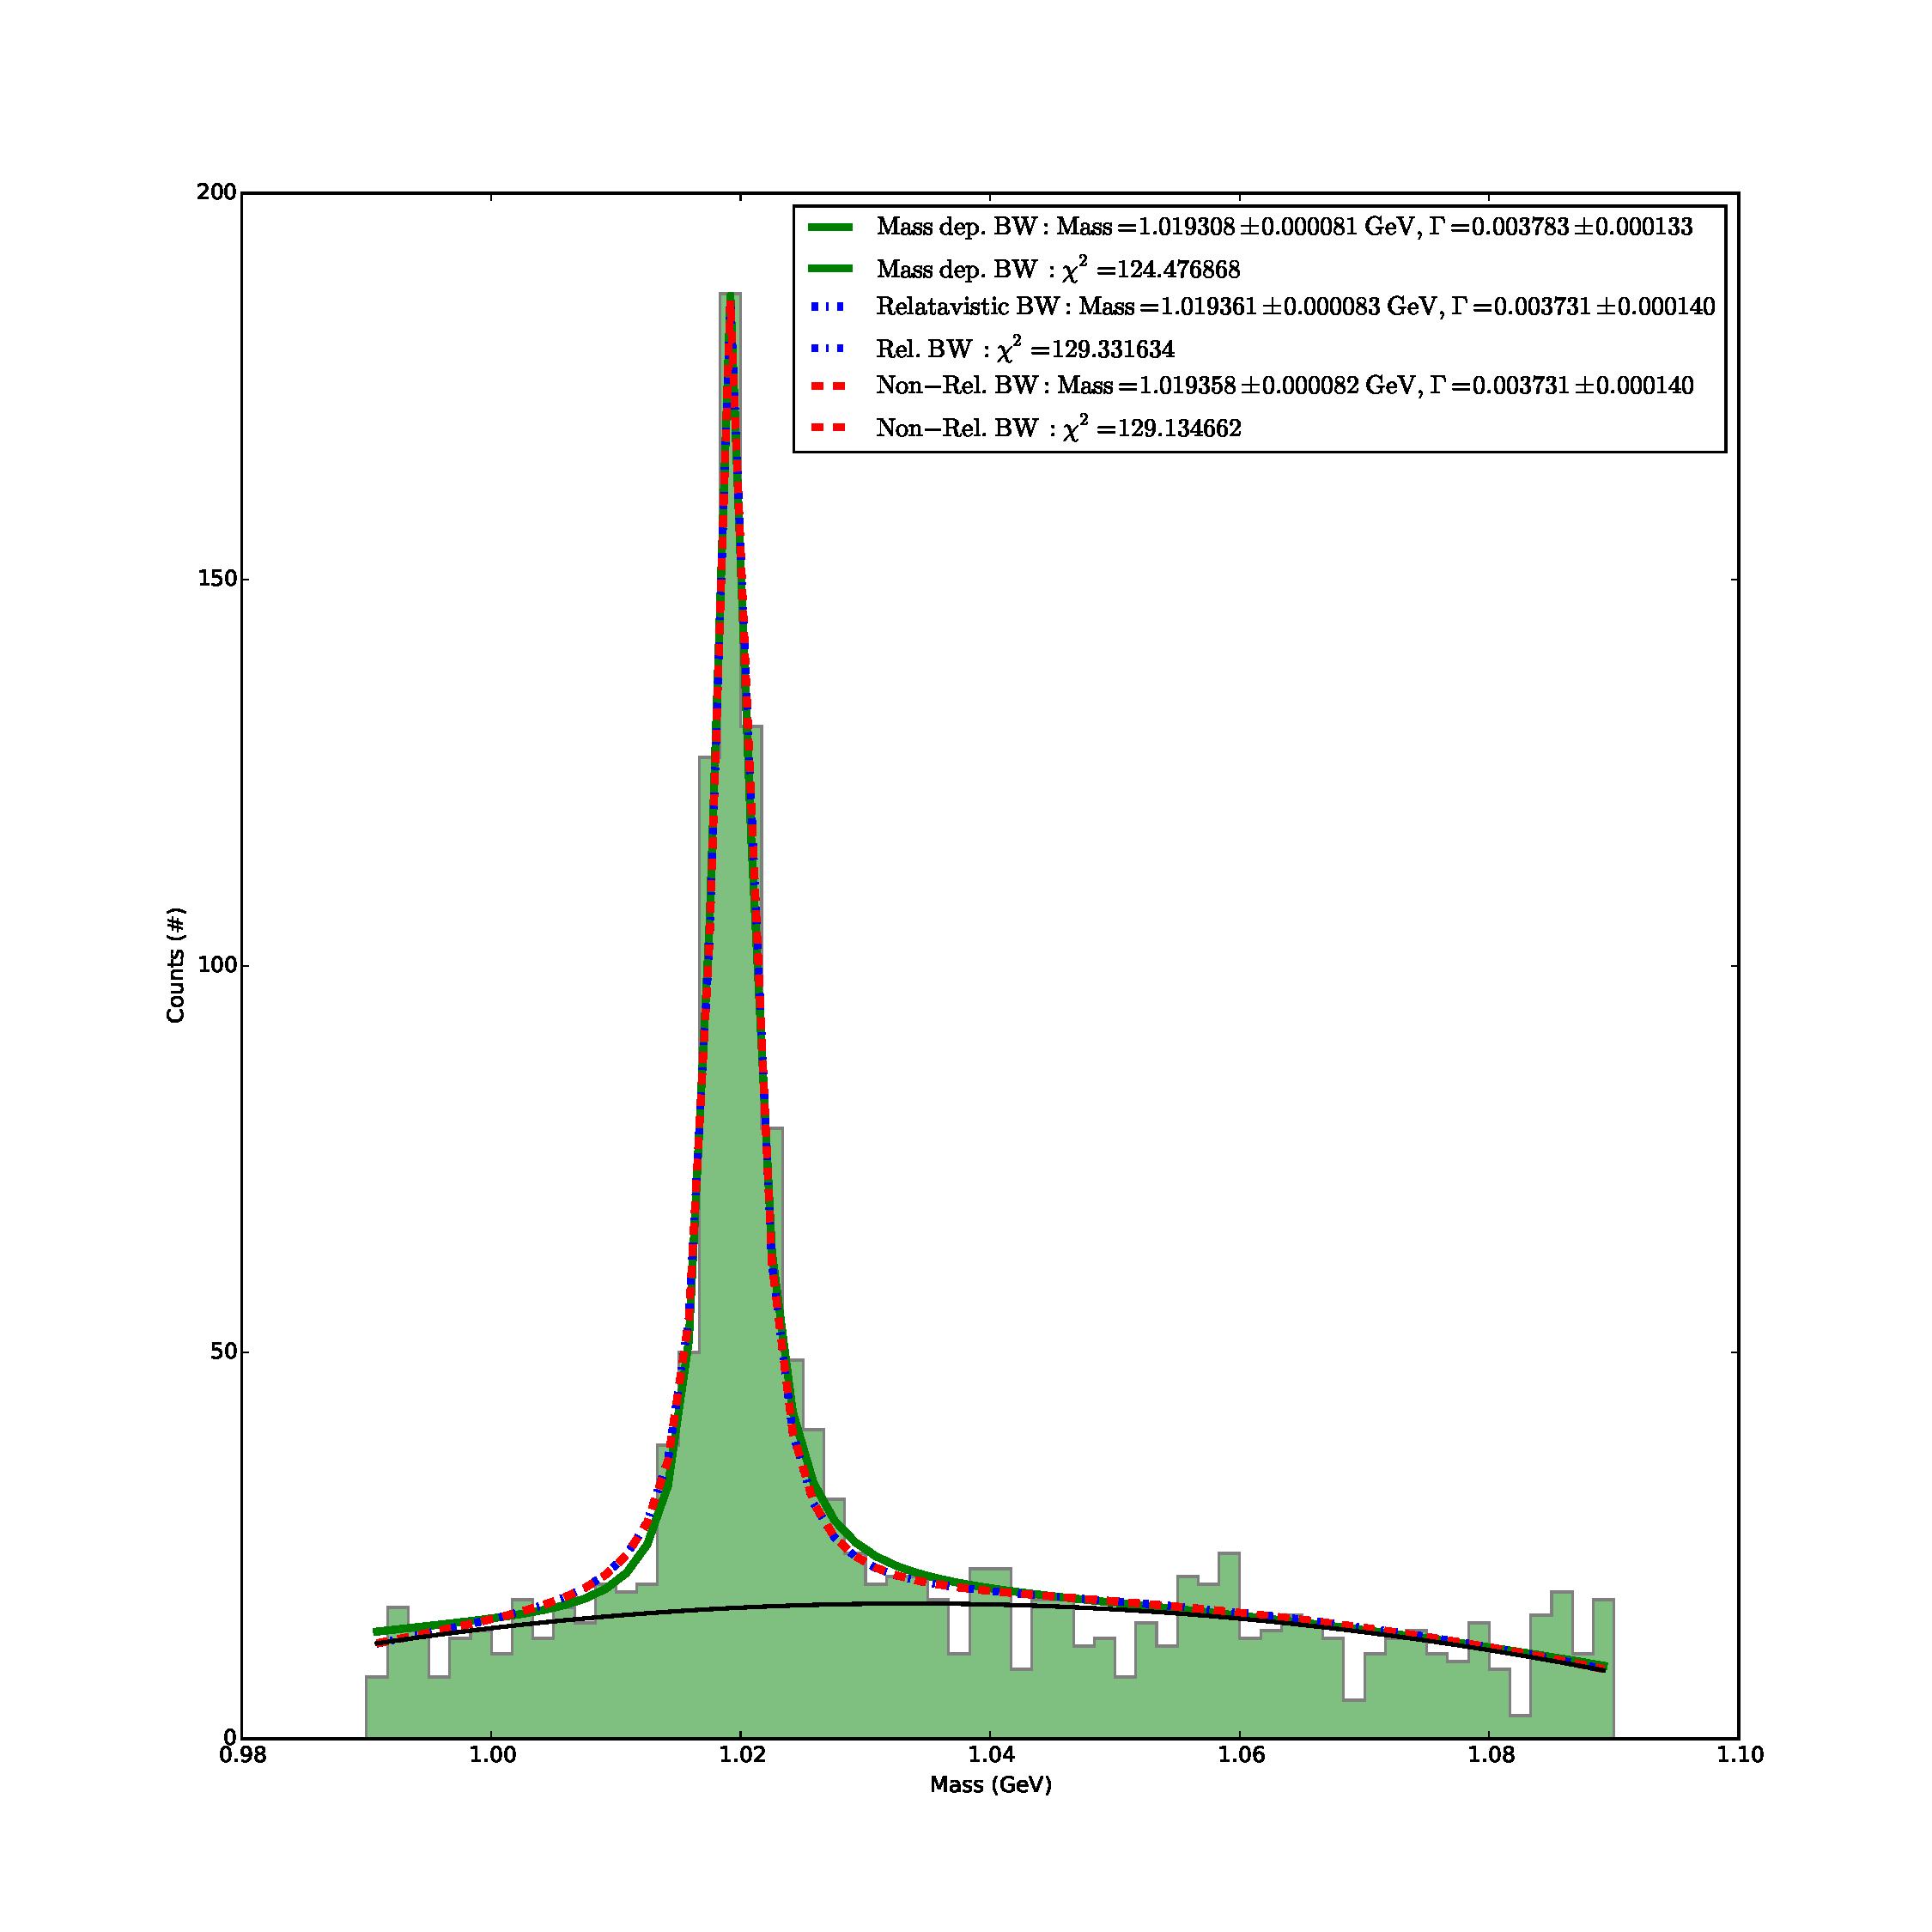
\includegraphics[scale=0.35]{Problem_3_withbackfit.pdf}
		\captionof{figure}{Three Breit-Wigner histograms with background for,
							$\phi \rightarrow K^{+} K^{-}$.
							The fit curves also include a fit for the background data giving a much better result
							as seen from the lower $\chi^2$ values.}

		\ \ \ \ \ With the background included into the fit, the $\chi^2$ values decrease showing the fit 
		becomes better.  With the background included the fits also find the correct peak as well as
		fit the tail better.  However with more data the fit would become even better.



\end{enumerate}

\end{document}
